\documentclass[11pt]{article}

\usepackage[margin=1in]{geometry}
\usepackage{amsmath, amssymb, amsthm}
\usepackage{graphicx}
\usepackage{hyperref}

\newtheorem{proposition}{Proposition}

\title{Projection--Carry Geometry of Polynomial Number Multiplication}
\author{Projection--Carry Geometry Project}
\date{\today}

\begin{document}

\maketitle

\begin{abstract}
We study base-\(B\) multiplication through a projection--carry decomposition.
Given digit polynomials \(X=\sum_i a_i B^i\) and \(Y=\sum_j b_j B^j\), their
product first forms an outer-product interaction matrix \(M_{ij}=a_i b_j\).
The raw product coefficients are obtained by diagonal projection,
\[
c_k=\sum_{i+j=k}M_{ij},
\]
which is equivalently the pushforward of the digit-interaction field under
\((i,j)\mapsto i+j\). These raw coefficients are then normalized by the
base-\(B\) carry recurrence. This separates multiplication into a bilinear
projection step and a nonlinear carry-flow step. We formalize carry as a
directed mass flow along the degree axis, prove a local carry activation law,
and introduce carry-complexity metrics including carry mass, carry count,
carry entropy, cascade length, and value-weighted carry. We further connect
carry behavior to digit-support geometry: the raw support is the sumset
\(S_X+S_Y\), and its representation counts bound the possible diagonal mass.
Synthetic scaling experiments show that additive energy and maximal
representation count are associated with carry mass, while sumset size and
support density are associated with carry count and cascade extent. The
framework is structural rather than algorithmic, providing a geometric lens on
polynomial number multiplication and carry propagation.
\end{abstract}

\section{Introduction}

Multiplication is usually treated as scalar arithmetic: two integers enter and
one integer exits. In a positional base, however, multiplication has internal
geometry. Digits occupy degree positions, digit pairs interact across a
two-dimensional index grid, and carry propagation moves excess mass along a
one-dimensional degree axis. Projection--Carry Geometry makes this structure
explicit.

Fix a base \(B\ge 2\). We write nonnegative integers as digit polynomials
\[
    X=\sum_i a_i B^i,\qquad
    Y=\sum_j b_j B^j,
\]
where \(0\le a_i,b_j<B\). The product is decomposed into three stages. First,
the digit interaction field is the outer-product matrix
\[
    M_{ij}=a_i b_j.
\]
Second, anti-diagonal projection aggregates interactions with the same total
degree,
\[
    c_k=\sum_{i+j=k}M_{ij}.
\]
Third, the raw coefficients \(c_k\) are converted into valid base-\(B\) digits
by carry normalization.

The main thesis is that base-\(B\) multiplication decomposes into bilinear
diagonal projection followed by nonlinear carry flow. The projection step is
ordinary convolution of digit polynomials. The carry step is a directed mass
flow along the degree axis, locally activated when \(c_k+r_k\ge B\), where
\(r_k\) is incoming carry.

This viewpoint separates potential interaction geometry from realized carry
behavior. If \(S_X=\{i:a_i\ne 0\}\) and \(S_Y=\{j:b_j\ne 0\}\), then the raw
support before carry is the sumset \(S_X+S_Y\). The representation counts
\[
    \rho_{X,Y}(k)=\#\{(i,j)\in S_X\times S_Y:i+j=k\}
\]
measure concentration of possible interactions on anti-diagonals. We argue
that this support-sumset geometry shapes carry complexity, while digit
amplitudes and incoming carry determine the realized local events.

The contributions are:
\begin{itemize}
    \item[C1.] A matrix projection formulation of positional multiplication.
    \item[C2.] A formulation of carry as nonlinear mass flow.
    \item[C3.] A local carry activation law.
    \item[C4.] Support-sumset geometry and representation-count bounds for raw
    diagonal mass.
    \item[C5.] Carry-complexity metrics and empirical scaling experiments.
\end{itemize}

This is a structural and geometric framework, not a new fast multiplication
algorithm. Its purpose is to expose the anatomy of multiplication and carry
propagation, not to replace existing arithmetic algorithms.

\section{Theorem Spine}

This section collects the definitions and elementary propositions used
throughout the paper.

\paragraph{Digit polynomials.}
For a base \(B\ge 2\), write
\[
    X=\sum_i a_i B^i,\qquad Y=\sum_j b_j B^j,
\]
where \(a_i,b_j\in\{0,1,\ldots,B-1\}\). The digit vectors are indexed from
low degree to high degree.

\paragraph{Interaction matrix.}
The digit interaction matrix is
\[
    M_{ij}=a_i b_j.
\]
It records the pairwise contribution of digit \(a_i\) and digit \(b_j\).

\paragraph{Diagonal projection.}
The raw diagonal coefficients are
\[
    c_k=\sum_{i+j=k} M_{ij}.
\]
Equivalently, diagonal projection pushes the matrix \(M\) forward under
\((i,j)\mapsto i+j\).

\paragraph{Carry normalization.}
Set \(r_0=0\). Carry normalization is defined by
\[
    s_k=c_k+r_k,\qquad
    d_k=s_k\bmod B,\qquad
    r_{k+1}=\left\lfloor \frac{s_k}{B}\right\rfloor.
\]
The output digits \(d_k\) satisfy \(0\le d_k<B\).

\begin{proposition}[Projection equals convolution]
The sequence \(c=(c_k)\) is the discrete convolution of the digit sequences
\(a=(a_i)\) and \(b=(b_j)\).
\end{proposition}

\begin{proof}
For every \(k\),
\[
    (a*b)_k=\sum_i a_i b_{k-i}=\sum_{i+j=k}a_i b_j=\sum_{i+j=k}M_{ij}=c_k.
\]
\end{proof}

\begin{proposition}[Carry preserves value]
If \(d\) is obtained from \(c\) by base-\(B\) carry normalization, then
\[
    \sum_k c_k B^k=\sum_k d_k B^k.
\]
\end{proposition}

\begin{proof}
The recurrence gives \(c_k+r_k=d_k+B r_{k+1}\). Multiplying by \(B^k\) and
summing over \(k\), the carry terms telescope. Since \(r_0=0\) and the final
carry is exhausted after finitely many positions, the two values are equal.
\end{proof}

\begin{proposition}[Local carry activation]
Outgoing carry at degree \(k\) is active if and only if
\[
    c_k+r_k\ge B.
\]
\end{proposition}

\begin{proof}
By definition \(r_{k+1}=\lfloor(c_k+r_k)/B\rfloor\). Because \(c_k+r_k\) is a
nonnegative integer, \(r_{k+1}>0\) exactly when \(c_k+r_k\ge B\).
\end{proof}

\paragraph{Digit support and support sumset.}
Define
\[
    S_X=\{i:a_i\ne 0\},\qquad S_Y=\{j:b_j\ne 0\},
\]
and
\[
    S_X+S_Y=\{i+j:i\in S_X,\ j\in S_Y\}.
\]

\paragraph{Representation count.}
For each degree \(k\), define
\[
    \rho_{X,Y}(k)=\#\{(i,j)\in S_X\times S_Y:i+j=k\}.
\]

\begin{proposition}[Raw support equals support sumset]
For nonnegative digits,
\[
    \operatorname{supp}(c)=S_X+S_Y.
\]
\end{proposition}

\begin{proof}
If \(k\in S_X+S_Y\), some supported pair \((i,j)\) satisfies \(i+j=k\), and
then \(a_i b_j>0\), so \(c_k>0\). Conversely, if \(c_k>0\), at least one
summand \(a_i b_j\) with \(i+j=k\) is positive, hence \(i\in S_X\) and
\(j\in S_Y\).
\end{proof}

\begin{proposition}[Representation-count bound]
For every degree \(k\),
\[
    c_k\le (B-1)^2\rho_{X,Y}(k).
\]
\end{proposition}

\begin{proof}
Each nonzero digit product is at most \((B-1)^2\), and there are
\(\rho_{X,Y}(k)\) support pairs on the anti-diagonal \(i+j=k\).
\end{proof}

\paragraph{Carry complexity metrics.}
We summarize carry flow by carry mass, carry count, carry depth, carry entropy,
maximum cascade length, carry amplification ratio, and value-weighted carry.
These metrics quantify the nonlinear normalization cost after bilinear
projection.

\section{Carry Normalization}

Raw coefficients $c_k$ need not be valid base-$B$ digits. Carry normalization
defines
\[
  s_k = c_k + r_k,\qquad d_k = s_k \bmod B,\qquad r_{k+1} = \left\lfloor \frac{s_k}{B} \right\rfloor,
\]
with $r_0=0$. The normalized result is
\[
  XY = \sum_k d_k B^k.
\]

This step is nonlinear because thresholding and integer division redistribute
mass along the degree axis.

\subsection{Carry as Nonlinear Mass Flow}

After diagonal projection, the product is represented by a sequence of raw
coefficients
\[
    c_k = \sum_{i+j=k} a_i b_j.
\]
These coefficients need not be valid base-\(B\) digits. We therefore define
carry normalization by the recurrence
\[
    r_0 = 0,
\]
\[
    s_k = c_k + r_k,
\]
\[
    d_k = s_k \bmod B,
\]
\[
    r_{k+1} = \left\lfloor \frac{s_k}{B} \right\rfloor.
\]
Here \(r_k\) is the incoming carry at degree \(k\), \(d_k\) is the normalized
digit kept at degree \(k\), and \(r_{k+1}\) is the outgoing carry transported
from degree \(k\) to degree \(k+1\).

This interpretation views carry as a directed mass flow along the degree axis:
\[
    k \longrightarrow k+1.
\]
The mass transported across this edge is \(r_{k+1}\). Thus diagonal projection
is a bilinear operation, while carry normalization is a nonlinear flow process.

\begin{proposition}[Value preservation of carry normalization]
Let \(c=(c_k)\) be a finite sequence of nonnegative integer raw coefficients.
Let \(d=(d_k)\) be obtained from \(c\) by base-\(B\) carry normalization. Then
\[
    \sum_k c_k B^k = \sum_k d_k B^k.
\]
\end{proposition}

\begin{proof}
By the carry recurrence,
\[
    c_k + r_k = d_k + B r_{k+1}.
\]
Multiplying by \(B^k\), we obtain
\[
    c_k B^k + r_k B^k = d_k B^k + r_{k+1}B^{k+1}.
\]
Summing over \(k\), the carry terms telescope. Since \(r_0=0\) and the final
carry is eventually exhausted, we get
\[
    \sum_k c_k B^k = \sum_k d_k B^k.
\]
\end{proof}

\section{Local Carry Laws}

Carry normalization is governed by a local threshold rule. At degree \(k\), let
\[
    s_k = c_k + r_k,
\]
where \(c_k\) is the raw coefficient and \(r_k\) is the incoming carry. Then
\[
    d_k = s_k \bmod B,\qquad
    r_{k+1} = \left\lfloor \frac{s_k}{B} \right\rfloor.
\]

\begin{proposition}[Local Carry Activation]
The outgoing carry at degree \(k\) is active if and only if
\[
    c_k + r_k \ge B.
\]
\end{proposition}

\begin{proof}
By definition,
\[
    r_{k+1} = \left\lfloor \frac{c_k+r_k}{B} \right\rfloor.
\]
Since \(c_k+r_k\) is a nonnegative integer and \(B\ge 2\), the floor is
positive exactly when \(c_k+r_k \ge B\). Thus \(r_{k+1}>0\) if and only if
\(c_k+r_k \ge B\).
\end{proof}

\paragraph{Carry cascade length.}
A carry cascade is a maximal consecutive block of active carry edges
\[
    k \to k+1.
\]
The cascade length is the number of active edges in such a block. The maximum
carry cascade length records the longest uninterrupted carry propagation event.

\paragraph{Value-weighted carry flow.}
The value-weighted carry flow is
\[
    \operatorname{VWC}(c) = \sum_k r_{k+1} B^{k+1}.
\]
It measures transported carry mass in positional value units rather than raw
edge-count units. A normalized version divides this quantity by
\(\max(\sum_k c_k B^k,1)\).

Carry is local in recurrence but global in consequence because outgoing carry
changes the next degree. Thus \(c_k\) alone does not determine activation:
the correct local state variable is \(s_k=c_k+r_k\).

\section{Support-Sumset Geometry}

\paragraph{Digit support.}
For a digit vector \(a=(a_i)\), its support is
\[
    S_X = \{i : a_i \ne 0\}.
\]
Similarly \(S_Y=\{j:b_j\ne 0\}\).

\paragraph{Support sumset.}
The support sumset is
\[
    S_X + S_Y = \{i+j : i\in S_X,\ j\in S_Y\}.
\]
It is the degree-level footprint of all possible digit interactions before
carry normalization.

\paragraph{Representation counts.}
For each degree \(k\), define
\[
    \rho_{X,Y}(k) = \#\{(i,j)\in S_X\times S_Y : i+j=k\}.
\]
The number \(\rho_{X,Y}(k)\) is the diagonal density of the support geometry. The
additive energy is
\[
    E(S_X,S_Y)=\sum_k \rho_{X,Y}(k)^2,
\]
which measures concentration of representation counts across anti-diagonals.

\begin{proposition}[Raw support as a sumset]
Assume the digits are nonnegative. Let
\[
    c_k=\sum_{i+j=k} a_i b_j.
\]
Then
\[
    \operatorname{supp}(c)=S_X+S_Y.
\]
\end{proposition}

\begin{proof}
If \(k\in S_X+S_Y\), then there exist \(i\in S_X\) and \(j\in S_Y\) with
\(i+j=k\). Since digits are nonnegative and supported digits are positive,
\(a_i b_j>0\), so \(c_k>0\). Conversely, if \(c_k>0\), at least one summand
\(a_i b_j\) with \(i+j=k\) is positive. Hence \(i\in S_X\), \(j\in S_Y\),
and \(k\in S_X+S_Y\).
\end{proof}

\begin{proposition}[Representation-count bound]
For base \(B\), every raw coefficient satisfies
\[
    c_k \le (B-1)^2 \rho_{X,Y}(k).
\]
\end{proposition}

\begin{proof}
Every digit product satisfies \(a_i b_j\le (B-1)^2\). At degree \(k\), there
are exactly \(\rho_k\) support pairs that can contribute nonzero products.
Summing these products gives the stated bound.
\end{proof}

Carry complexity is influenced by concentration of \(\rho_{X,Y}(k)\). Large
representation counts and high additive energy indicate many support-pair
collisions on the same anti-diagonals, increasing the potential raw mass that
carry normalization must absorb. The realized carry still depends on digit
values and incoming carry, but support-sumset geometry provides a structural
predictor for where nonlinear normalization may become active.

\section{Empirical Scaling Experiments}

\paragraph{Experimental setup.}
The synthetic scaling experiments sample random digit supports and digit
amplitudes across bases \(B\in\{2,10,16\}\), digit lengths such as \(8\) and
\(16\) in the default reproducible grid, and support densities
\(\{0.2,0.5,0.7,1.0\}\). For each configuration, random pairs are generated
and passed through the projection--carry pipeline. The generated summary and
correlation tables are stored in the \texttt{paper/tables} directory.

\paragraph{Predictors and outcomes.}
The geometry predictors are sumset size, maximum representation count,
additive energy, support densities, and diagonal mass concentration. The carry
outcomes are carry mass, carry count, maximum carry cascade length, carry
amplification ratio, and normalized value-weighted carry. We also examine
normalized quantities such as carry mass per digit and cascade fraction.

\paragraph{Raw support concentration and carry mass.}
Figure~\ref{fig:additive-energy-carry-mass} shows additive energy against
carry mass. Additive energy measures concentration of representation counts on
anti-diagonals; high energy indicates that many support pairs may collide on a
small set of degrees. Figure~\ref{fig:max-rep-carry-mass} gives the related
view using the largest representation count. In the synthetic grid, both
quantities behave as structural predictors for absolute carry mass.

\begin{figure}[ht]
    \centering
    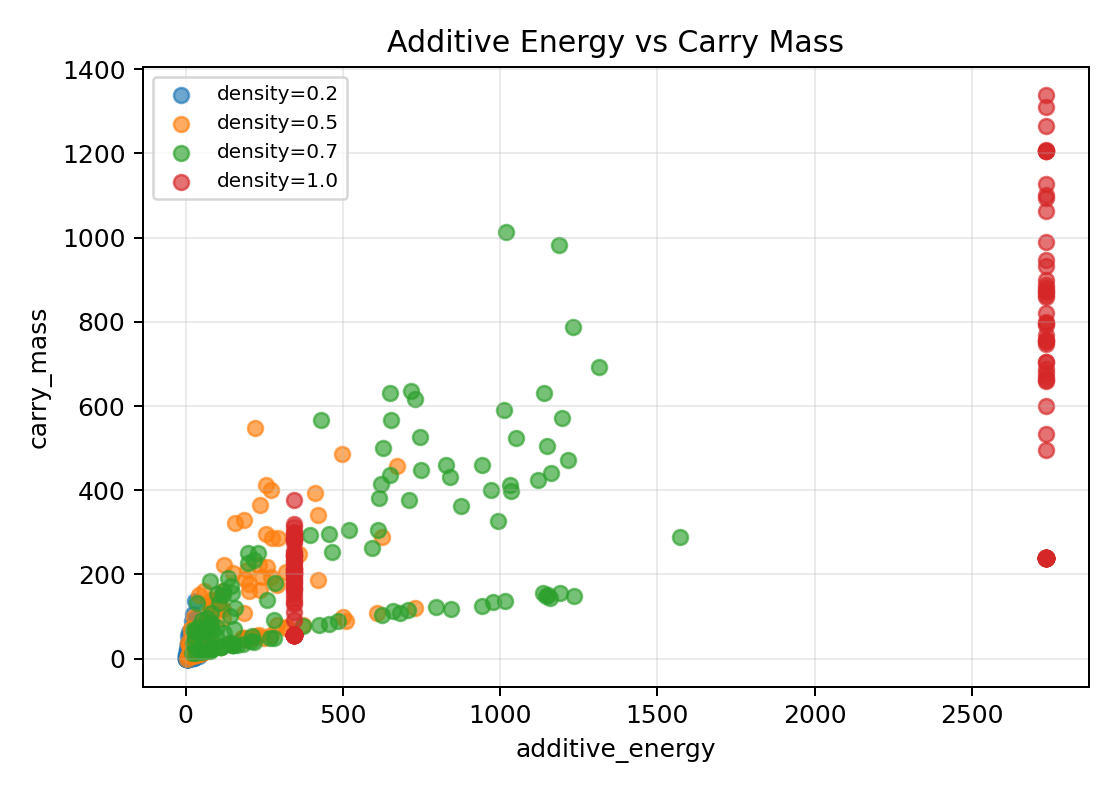
\includegraphics[width=0.78\linewidth]{figures/additive_energy_vs_carry_mass.png}
    \caption{Additive energy versus carry mass.}
    \label{fig:additive-energy-carry-mass}
\end{figure}

\begin{figure}[ht]
    \centering
    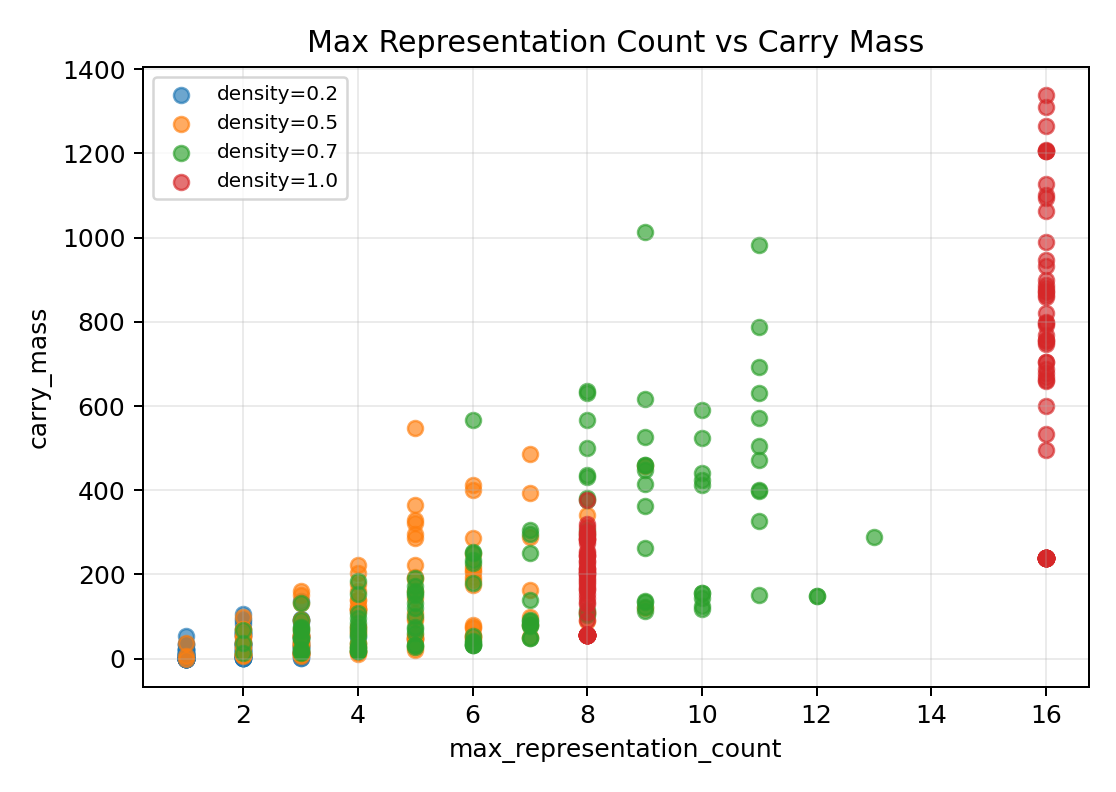
\includegraphics[width=0.78\linewidth]{figures/max_representation_vs_carry_mass.png}
    \caption{Maximum representation count versus carry mass.}
    \label{fig:max-rep-carry-mass}
\end{figure}

\paragraph{Spatial extent of carry flow.}
Figure~\ref{fig:sumset-carry-count} compares sumset size with carry count.
Sumset size tracks how many degree positions can receive raw mass; this is
therefore related to the spatial extent of carry activity. Figure~\ref{fig:density-cascade}
shows that support density is associated with cascade fraction, the normalized
length of the longest consecutive active-carry segment.

\begin{figure}[ht]
    \centering
    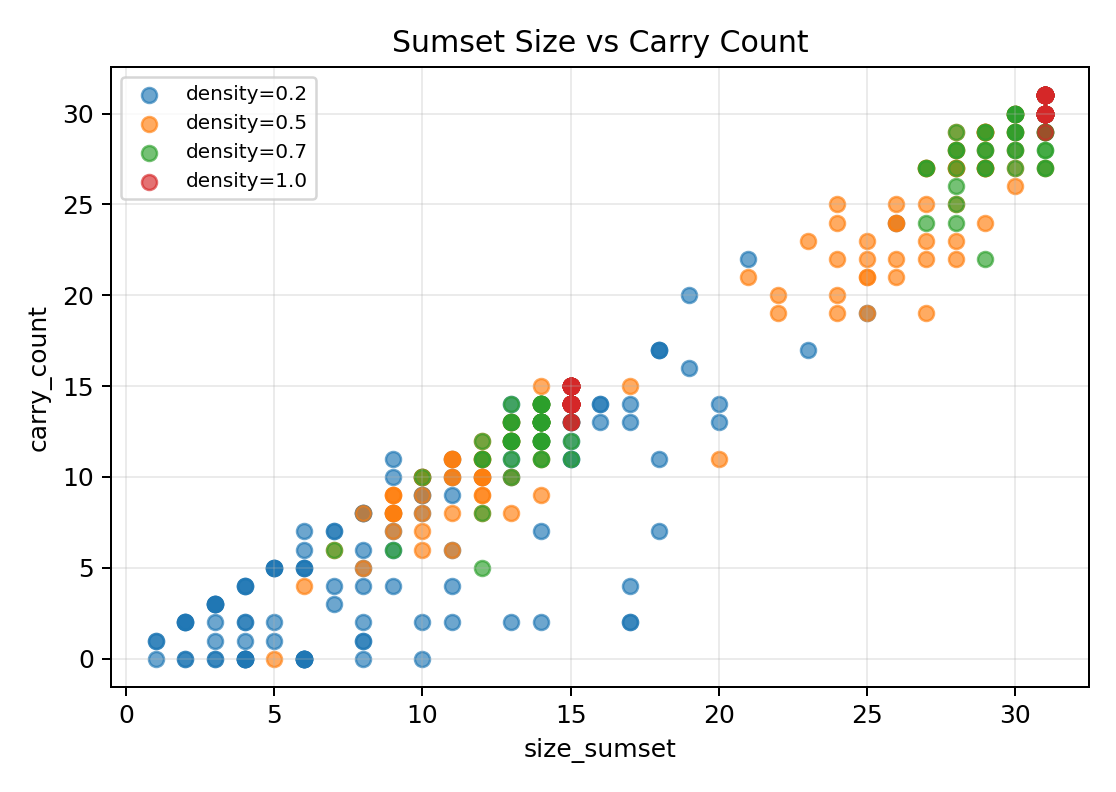
\includegraphics[width=0.78\linewidth]{figures/size_sumset_vs_carry_count.png}
    \caption{Support-sumset size versus carry count.}
    \label{fig:sumset-carry-count}
\end{figure}

\begin{figure}[ht]
    \centering
    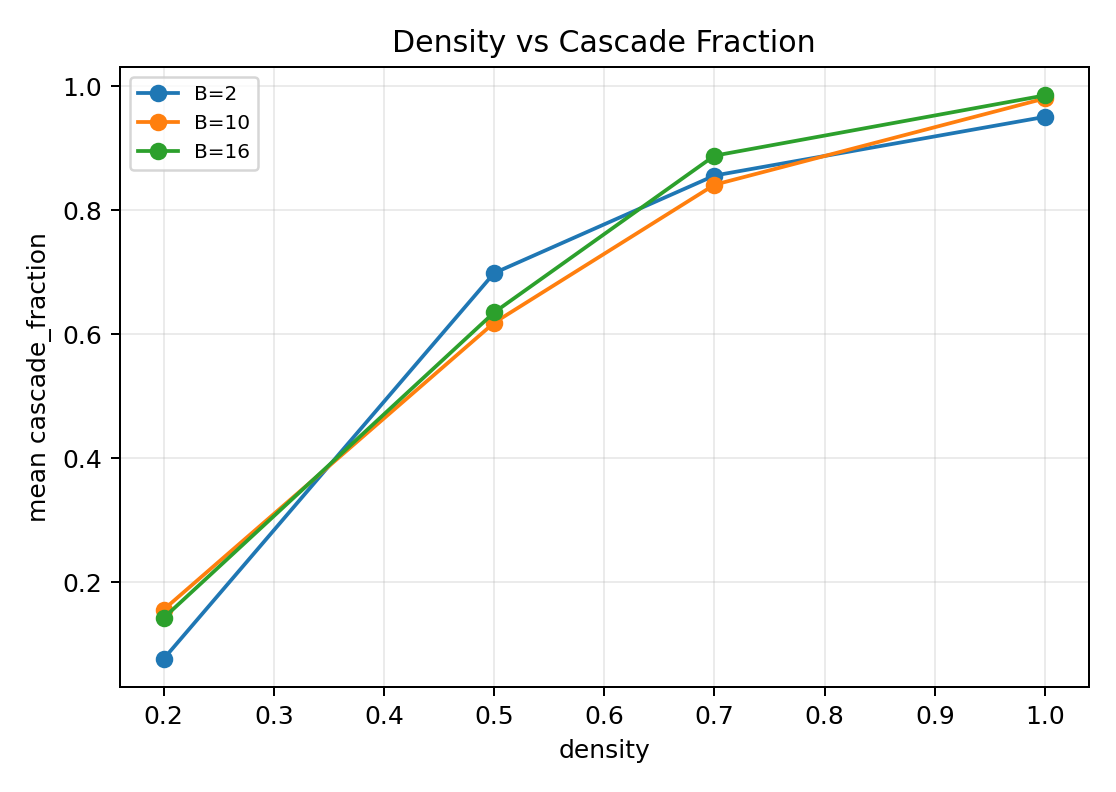
\includegraphics[width=0.78\linewidth]{figures/density_vs_cascade_fraction.png}
    \caption{Support density versus cascade fraction.}
    \label{fig:density-cascade}
\end{figure}

\paragraph{Base effects and normalized metrics.}
Base affects absolute carry mass and normalized amplification differently.
Figure~\ref{fig:base-amplification} shows carry amplification by base, while
Figure~\ref{fig:base-carry-mass-per-digit} shows carry mass per digit. Larger
bases raise the local activation threshold but also allow larger digit
products. The normalized plots should therefore be read together with the raw
plots rather than as replacements.

\begin{figure}[ht]
    \centering
    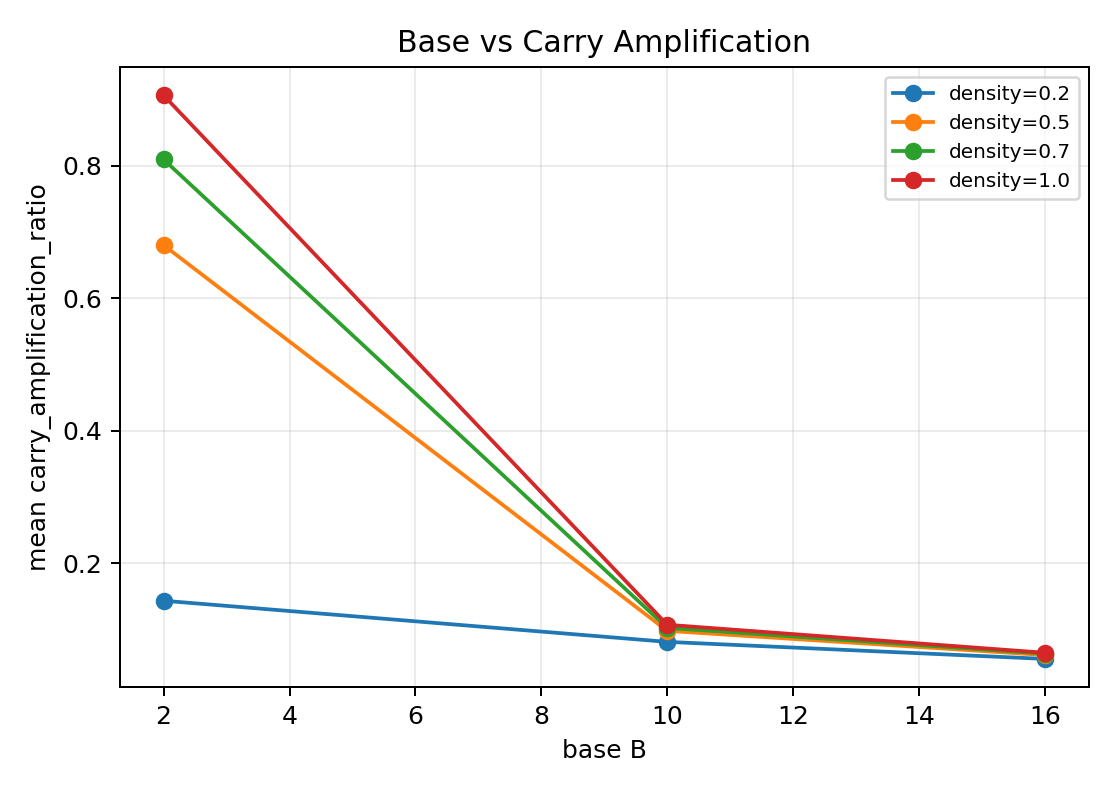
\includegraphics[width=0.78\linewidth]{figures/base_vs_carry_amplification.png}
    \caption{Base versus carry amplification ratio.}
    \label{fig:base-amplification}
\end{figure}

\begin{figure}[ht]
    \centering
    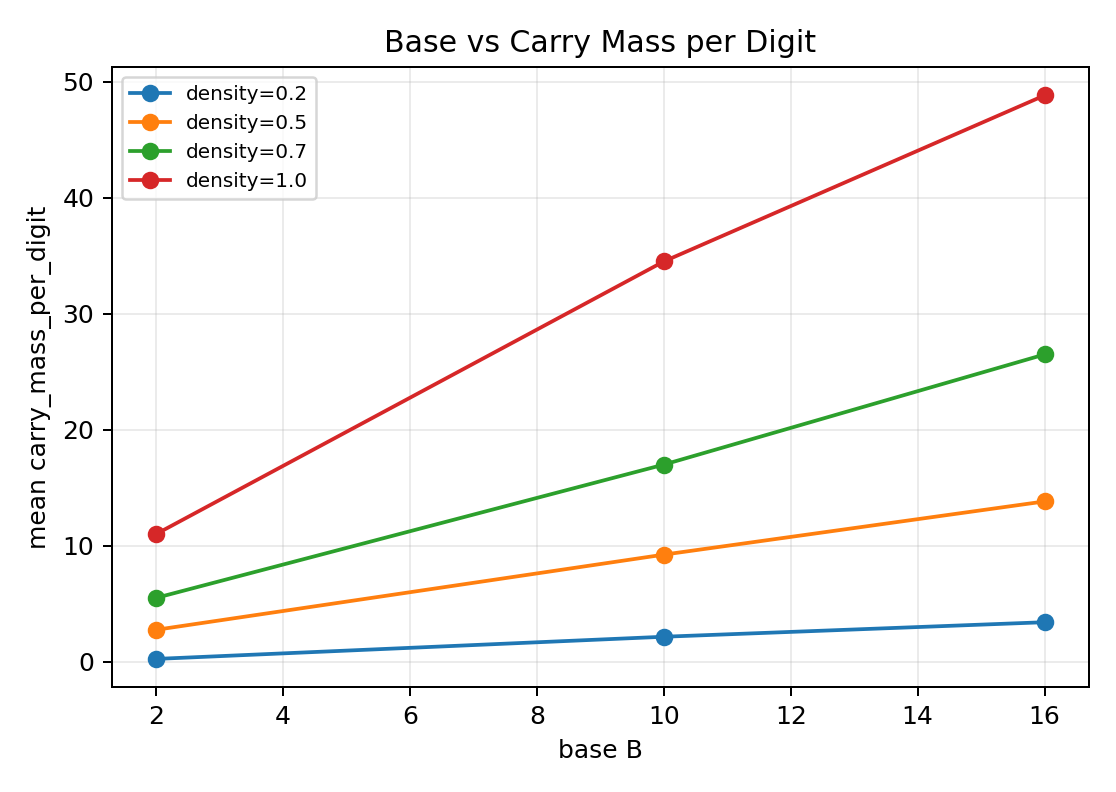
\includegraphics[width=0.78\linewidth]{figures/base_vs_carry_mass_per_digit.png}
    \caption{Base versus carry mass per digit.}
    \label{fig:base-carry-mass-per-digit}
\end{figure}

\paragraph{Interpreting normalization.}
Figure~\ref{fig:normalized-energy} shows normalized additive energy against
carry mass per digit. Normalized additive energy alone is insufficient because
it removes scale: two supports can have similar normalized concentration but
very different total interaction mass. This reinforces the central
interpretation: support geometry gives potential concentration, while digit
amplitudes and incoming carry determine realized carry flow.

\begin{figure}[ht]
    \centering
    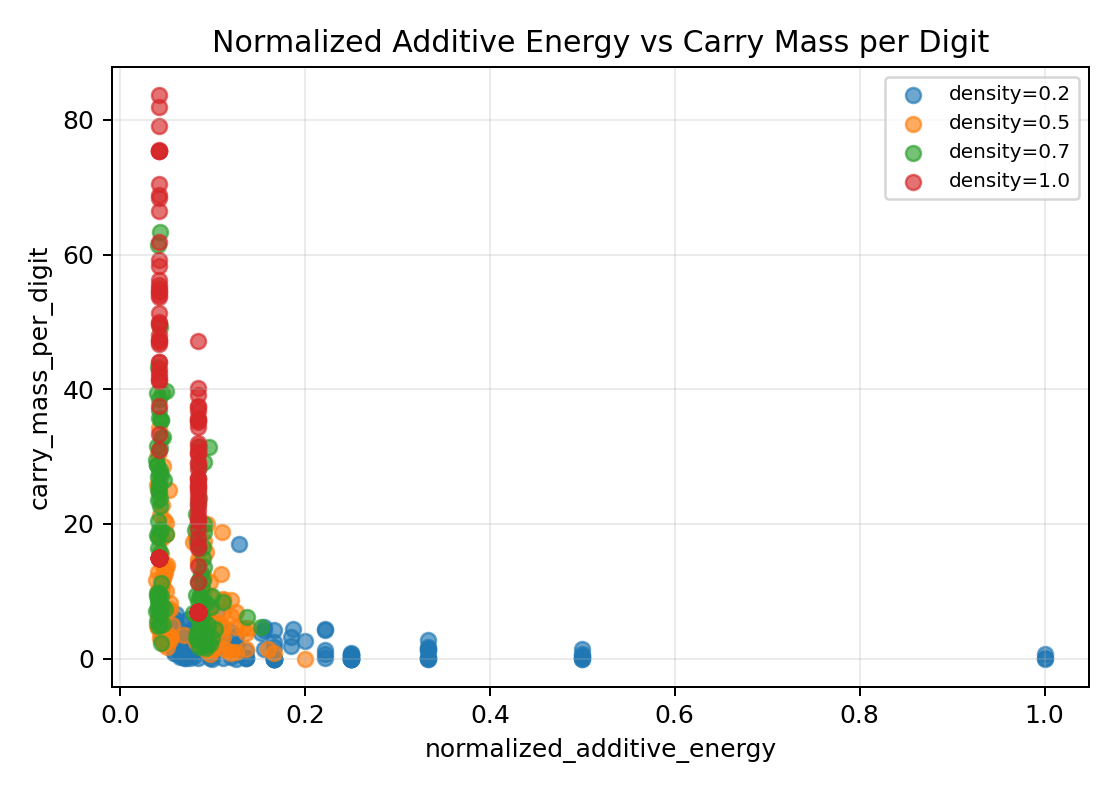
\includegraphics[width=0.78\linewidth]{figures/normalized_additive_energy_vs_carry_mass_per_digit.png}
    \caption{Normalized additive energy versus carry mass per digit.}
    \label{fig:normalized-energy}
\end{figure}

\section{Discussion and Limitations}

Projection--Carry Geometry is not a new multiplication algorithm. It is a
structural and geometric framework for the ordinary base-\(B\) multiplication
process. The goal is to separate bilinear projection from nonlinear carry flow
and to make the geometry of carry propagation measurable.

Support geometry controls potential mass concentration, not exact carry. The
sumset \(S_X+S_Y\), representation counts \(\rho_{X,Y}(k)\), and additive
energy describe where digit interactions can collide. They do not determine
the actual raw coefficient values. Digit amplitudes determine \(c_k\), and
incoming carry determines the realized activation condition \(c_k+r_k\ge B\).
Thus carry is locally activated but globally propagated through the recurrence.

The experiments are synthetic random digit experiments. They are useful for
testing structural hypotheses and producing reproducible scaling tables, but
they do not characterize every input distribution that appears in arithmetic
software or hardware. Deterministic support families may display different
behavior.

Normalized metrics must also be interpreted carefully. Normalization by digit
length, support size, or total interaction count can remove the scale that
drives absolute carry mass. For this reason, normalized figures should be read
alongside raw carry and raw support-concentration plots.

Future work includes binary multiplication and bit-level circuits,
multi-factor tensor projection, signed digits, negative coefficients, carry
minimization, and more direct connections to additive combinatorics.

\section{Conclusion}

Base-\(B\) multiplication can be viewed as bilinear projection followed by
nonlinear carry flow. The outer-product matrix records pairwise digit
interactions, anti-diagonal projection aggregates those interactions into raw
degree coefficients, and carry normalization transports excess mass along the
degree axis while preserving numerical value.

Carry is locally activated, globally propagated, and geometrically
conditioned. It is locally activated by the threshold \(c_k+r_k\ge B\), globally
propagated because outgoing carry changes the next degree, and geometrically
conditioned because support-sumset representation counts control where raw mass
can concentrate. This gives a coherent language for studying multiplication as
projection followed by normalization, and for relating carry complexity to the
geometry of digit supports.


\nocite{*}
\bibliographystyle{plain}
\bibliography{refs}

\end{document}
